\section*{Ejercicio 1}
\graphicspath{{Figuras/ej_01/}}

Comenzamos simulando la dinámica de dos neuronas Hogdkin-Huxley \cite{HH} conectadas simétricamente con interacciones sinapticas excitatorias e inhibitorias. Se utilizo una corriente externa $I_{\text{ext}}=10\,\text{mA}$ de manera que las neuronas estén oscilando periódicamente. La corriente de interacción sinaptica esta dada por
\begin{equation}
    I_{syn}(t) = -g_{syn} s(t) (V-V_{syn}),
\end{equation}
donde
\begin{align}
    \frac{ds}{dt}&= \frac{s_\infty(V) - s}{\tau}\\
    s_\infty(V)&= 0.5(1+\text{tanh}(\nicefrac{V}{5})),
\end{align}
siendo $V$ es el potencial de  la neurona y $\tau$ es el tiempo característico asociado a la inhibición, el cual se tomo como $\tau = 3\,\text{ms}$ durante todo el trabajo.

\begin{figure}[hb!]
    \centering
    \begin{subfigure}[b]{0.48\textwidth}
        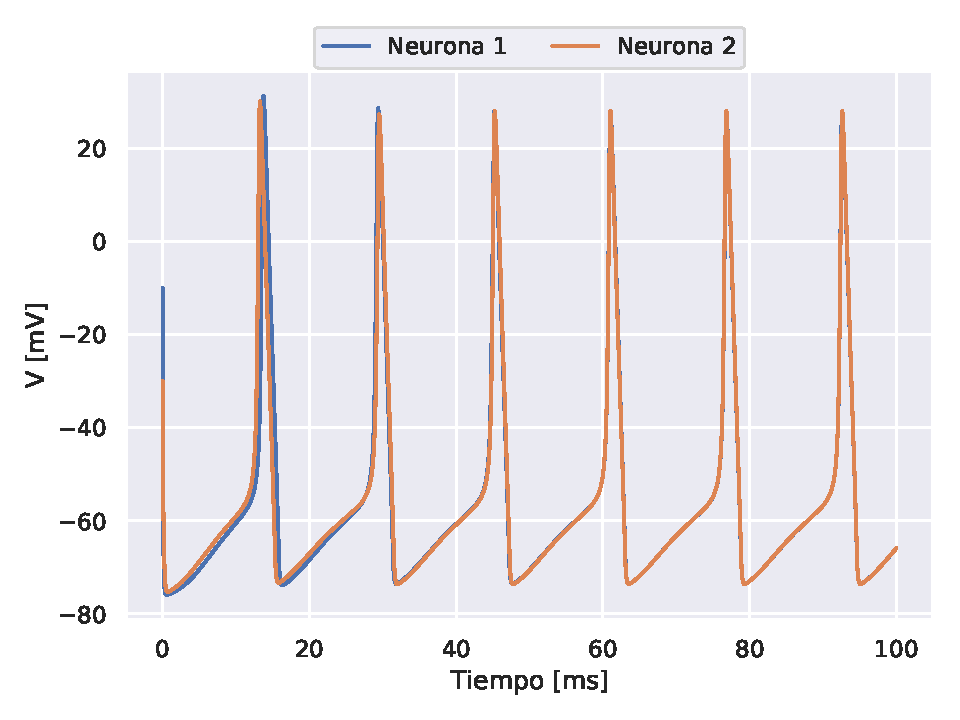
\includegraphics[width=\textwidth]{Excitatorio_inicio.pdf}
        \caption{}
        \label{Simulacion_Excitatorio_inicio}
    \end{subfigure}
    \hfill
    \begin{subfigure}[b]{0.48\textwidth}
        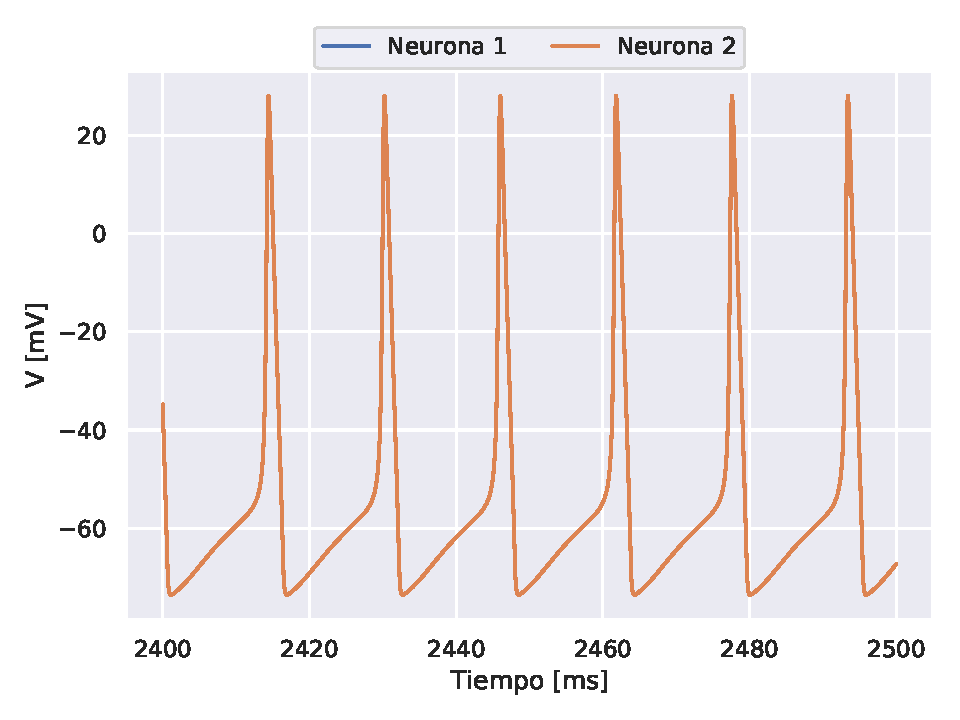
\includegraphics[width=\textwidth]{Excitatorio_final.pdf}
        \caption{}
        \label{Simulacion_Excitatorio_final}
    \end{subfigure}
    \caption{Simulación de la interacción excitatoria entre dos neuronas para $V_{syn}=0\,\text{mV}$ y $g_{syn}=1\,\frac{\text{mS}}{\text{cm}^2}$. En (a) se observan los primeros $100\,\text{ms}$ de la simulación, correspondiente al un régimen transitorio. Luego, en (b), se observa los últimos $100\,\text{ms}$ de la simulación, en donde el sistema se encuentra en un régimen estacionario y los spikes se encuentran en fase.}
    \label{ej01:Simulacion_Excitatorio}
\end{figure}

En las Figuras \ref{ej01:Simulacion_Excitatorio} se observan las evoluciones temporales del potencial de ambas neuronas, para el caso excitatorio ($V_{syn}=0$) e inhibitorio ($V_{syn}=-80$) respectivamente, tomando en $g_{syn} = 1\,\frac{\text{mS}}{\text{cm}^2}$. En ambos casos, la dinámica viene dada por un transitorio y luego del mismo se observa que los spikes de las neuronas se encuentran en fase para el caso excitatorio. Por otro lado, para la interacción inhibitoria, una vez alcanzado el régimen estacionario, dichos spikes se desfasan. El tiempo necesario para alcanzar el régimen estacionario depende del valor de $g_{syn}$.



\begin{figure}[h!]
    \centering
    \begin{subfigure}[b]{0.48\textwidth}
        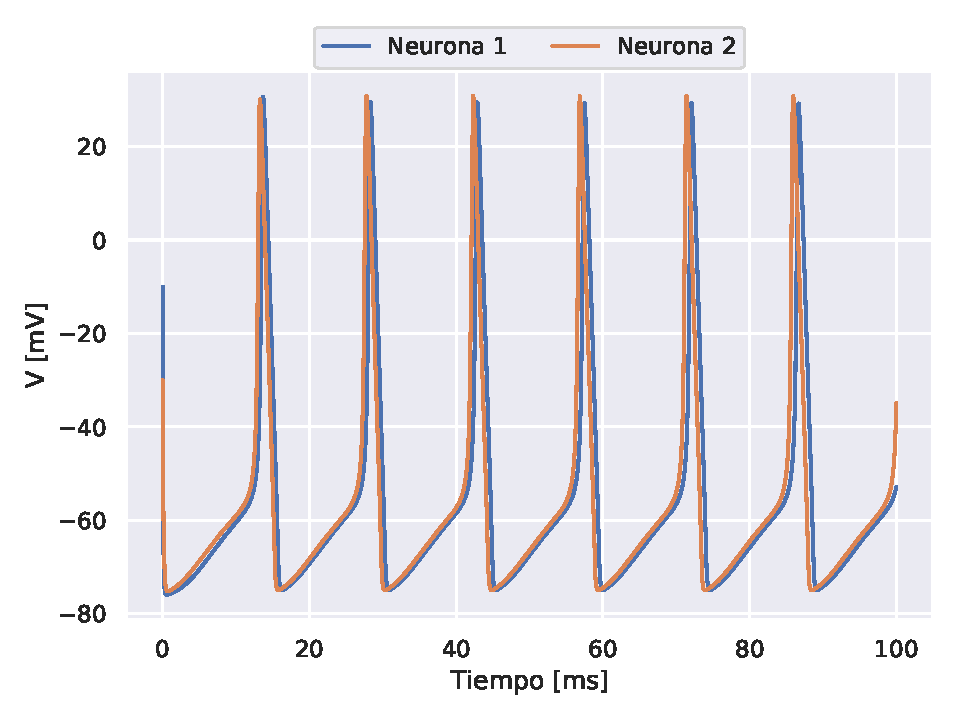
\includegraphics[width=\textwidth]{Inhibitorio_inicio.pdf}
        \caption{}
        \label{Simulacion_Inhibitorio_inicio}
    \end{subfigure}
    \hfill
    \begin{subfigure}[b]{0.48\textwidth}
        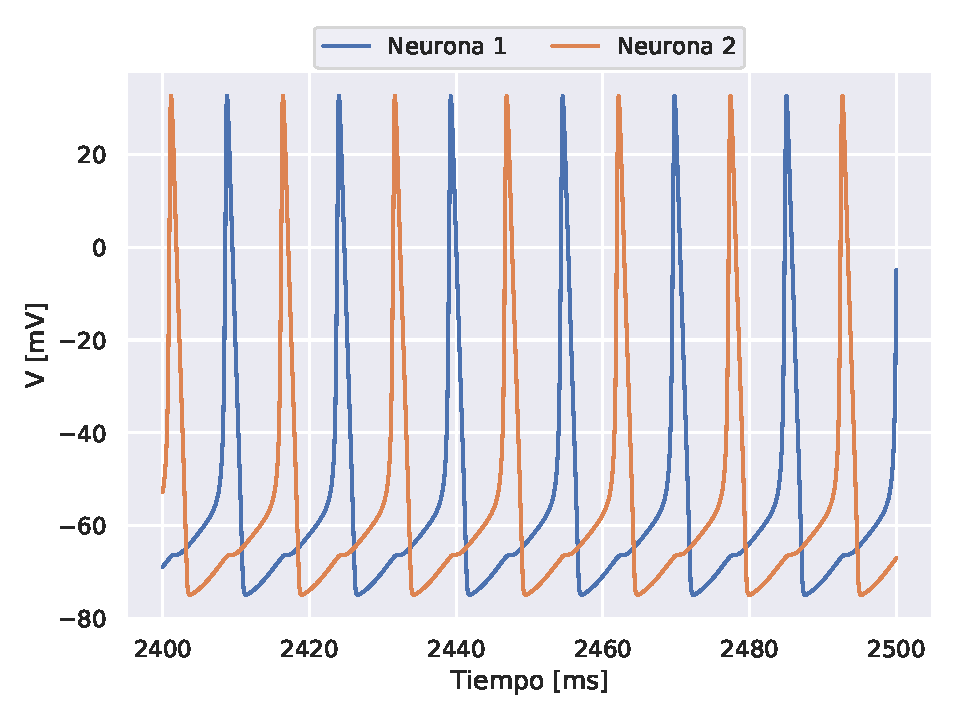
\includegraphics[width=\textwidth]{Inhibitorio_final.pdf}
        \caption{}
        \label{Simulacion_Inhibitorio_final}
    \end{subfigure}
    \caption{Simulación de la interacción inhibitoria entre dos neuronas para $V_{syn}=-80\,\text{mV}$ y $g_{syn}=1\,\frac{\text{mS}}{\text{cm}^2}$. En (a) se observan los primeros $100\,\text{ms}$ de la simulación, correspondiente al un régimen transitorio. Luego, en (b), se observa los últimos $100\,\text{ms}$ de la simulación, en donde el sistema se encuentra en un régimen estacionario y los spikes se encuentran desfasados.}
    \label{ej01:Simulacion_Inhibitorio}
\end{figure}


Se busco estudiar en detalle este desfasaje entre las neuronas y la tasa de disparo del sistema como función del parámetro $g_{syn}$ para valores entre $0$ y $2\,\frac{\text{mS}}{\text{cm}^2}$. Este estudio realizo tanto para interacciones excitatorias como inhibitorias, tomando $V_{syn}=0\,\text{mV}$ y $V_{syn}=-80\,\text{mV}$ respectivamente.


\begin{figure}[h!]
    \centering
    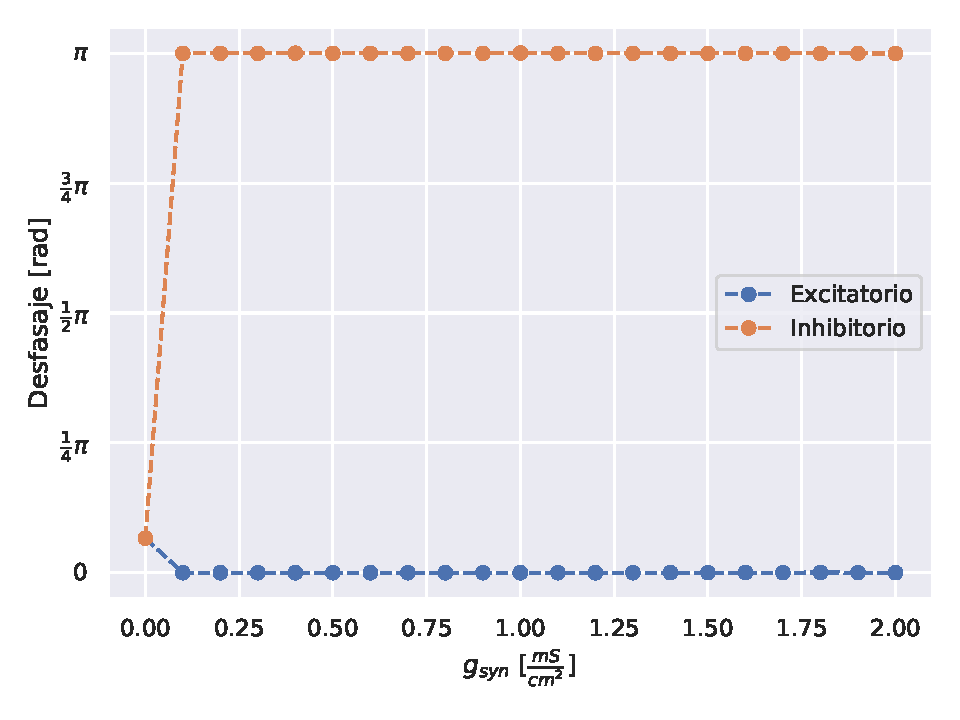
\includegraphics[width=0.6\textwidth]{Desfasaje.pdf}
    \caption{Desfasaje entre los spikes de las neuronas como función del parámetro $g_{syn}$ para la interacción excitatoria e inhibitoria. El desfasaje es calculado una vez alcanzado el régimen estacionario. Cuando la interacción entre neuronas no es nula (es decir, cuando $g_{syn} \neq 0$) se observa ua clara diferencia entre los desfasajes de las neuronas, siendo nulo para la interacción excitatoria, ya que la misma produce el efecto de acercar los spikes. Por otro lado, para la interacción inhibitoria, el desfasaje es de $\pi$, consecuencia de que la interacción inhibitoria produce el efecto de alejar los spikes de cada neurona.}
    \label{ej01:Desfasaje}
\end{figure}

\begin{figure}[h!]
    \centering
    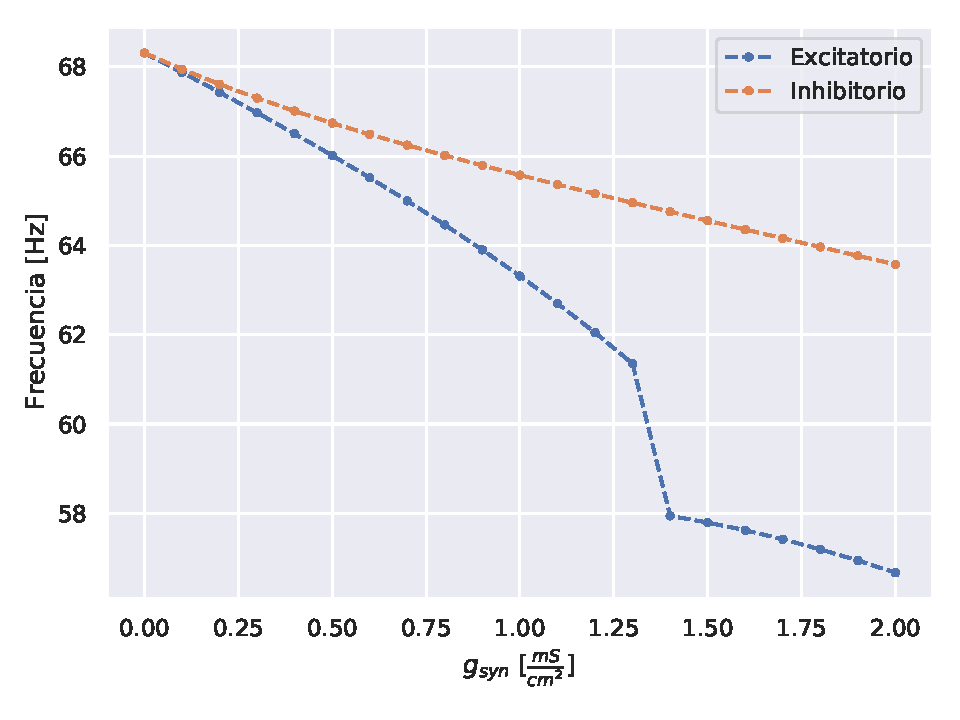
\includegraphics[width=0.6\textwidth]{Tasa_de_Disparo.pdf}
    \caption{Frecuencia entre los spikes de las neuronas como función del parámetro $g_{syn}$ para la interacción excitatoria e inhibitoria. La frecuencia es calculada una vez alcanzado el régimen estacionario. En ambos casos se observa que la tasa de disparo disminuye al aumentar $g_{syn}$}
    \label{ej01:tasaDeDisparo}
\end{figure}

En la Figura \ref{ej01:Desfasaje} se observa el desfasaje en función de $g_{syn}$ tanto para la interacción excitatoria como inhibitoria. El desfasaje es calculado una vez alcanzado el régimen estacionario. Cuando la interacción entre neuronas no es nula (es decir, cuando $g_{syn} \neq 0$) se observa ua clara diferencia entre los desfasajes de las neuronas, siendo nulo para la interacción excitatoria, ya que la misma produce el efecto de acercar los spikes. Por otro lado, para la interacción inhibitoria, el desfasaje es de $\pi$, consecuencia de que la interacción inhibitoria produce el efecto de alejar los spikes de cada neurona.

En la Figura \ref{ej01:tasaDeDisparo} se observa la frecuencia del sistema acoplado como función del parámetro $g_{syn}$, el cual influye en la intensidad de la interacción. Se observa la disminución de la frecuencia de las neuronas con el aumento del valor de $g_{syn}$. Para la curva correspondiente a la interacción excitatoria, esta disminución se debe a que la corriente $g_{syn}$ disminuye la corriente total dentro de la neurona. Por otro lado, para la interacción excitatoria, se observa que la disminución de la frecuencia es menos pronunciada, ya que el potencial inhibitorio ralentiza la frecuencia de los spikes de las neuronas, desfasandolos.